\documentclass[18pt]{article}
\usepackage[a4paper, total={6.5in, 8.5in}]{geometry}
\usepackage[linesnumbered,ruled,vlined]{algorithm2e}
\usepackage{caption}
\usepackage{subcaption}
\usepackage{amsmath}
\usepackage{tikz}


% Define colors
\definecolor{myblue}{RGB}{0, 102, 204}
\definecolor{mygreen}{RGB}{0, 153, 0}


% Declare lengths

\setlength{\parskip}{1em}

\newlength{\leafnodewidth} 
\newlength{\leafnodeheightone} 
\newlength{\leafnodeheighttwo}
\newlength{\leafnodetextstart}
\newlength{\leafnodetextend}

\newlength{\internalnoderadius}

\newlength{\leveldistance}

% Set length values

\setlength{\leafnodewidth}{6mm}
\setlength{\leafnodeheightone}{3mm}
\setlength{\leafnodeheighttwo}{9mm} 

\setlength{\leafnodetextstart}{11mm}
\setlength{\leafnodetextend}{15mm}

\setlength{\internalnoderadius}{3.5mm}

\setlength{\leveldistance}{14mm}

% Declare colors
\definecolor{leafcolorone}{RGB}{255,0,0} % red
\definecolor{leafcolortwo}{RGB}{0,0,255} % blue
\definecolor{internalnodecolor}{RGB}{0,255,0} % green
\definecolor{highlightededgecolor}{RGB}{139,1,102} %dark magenta
\definecolor{codecolorone}{RGB}{139,1,102} %dark magenta
\definecolor{codecolortwo}{RGB}{45, 141, 38} % dark green
\definecolor{dimcolor}{RGB}{217, 217, 217}


% Define the \leafnode command
\newcommand{\leafnode}[6]{
	\begin{tikzpicture}
		\filldraw[color=#1!90, fill=#1!3, thick, font=\tiny] (0,0) rectangle (\leafnodewidth, -\leafnodeheightone) node[midway, text=#3] {#4};
		\filldraw[color=#2!90, fill=#2!3, thick, font=\small] (0,-\leafnodeheightone) rectangle (\leafnodewidth, -\leafnodeheighttwo) node[midway, text=#3] {#5};
		
		% the following portion is only for showing after demonstration
		
		%\filldraw[color=white!100, fill=white!100, thick, font=\scriptsize] (0,-\leafnodetextstart) rectangle (\leafnodewidth, -\leafnodetextend) node[midway, text=#3] {#6};
		
	\end{tikzpicture}
}


% Define the \leafnode command
\newcommand{\labelledleafnode}[6]{
	\begin{tikzpicture}
		\filldraw[color=#1!90, fill=#1!3, thick, font=\tiny] (0,0) rectangle (\leafnodewidth, -\leafnodeheightone) node[midway, text=#3] {#4};
		\filldraw[color=#2!90, fill=#2!3, thick, font=\small] (0,-\leafnodeheightone) rectangle (\leafnodewidth, -\leafnodeheighttwo) node[midway, text=#3] {#5};
		
		\filldraw[color=violet!100, fill=white!100, thick, font=\scriptsize] (0,-\leafnodetextstart) rectangle (\leafnodewidth, -\leafnodetextend) node[midway, text=#3] {#6};
		
	\end{tikzpicture}
}

% Define the \internalnode command with a color argument
\newcommand{\internalnode}[3]{
	\begin{tikzpicture}
		\filldraw[color=#1!90, fill=#1!5, thick, font=\scriptsize] (0,0) circle (\internalnoderadius) node[midway, text=#2] {#3};
	\end{tikzpicture}
}


% Minimum Indicator
\newcommand{\mindicator}[0]{
	
	\vspace{0.5mm}
	
	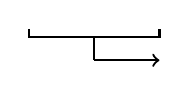
\begin{tikzpicture}
		
		\draw[black, thick] (0,0.1) -- (0,0) -- (1.66,0) -- (1.66,0.1);
		\draw[black, thick] (0.83,0) -- (0.83,-0.3);
		\draw[black, thick, ->] (0.83,-0.3) -- (1.66,-0.3);
		% Adding a dummy line for better positioning of the text
		\draw[white] (0,-0.4) -- (1.66,-0.4);
		
		
	\end{tikzpicture}
	\footnotesize{Minimum-weighted two nodes}
	
}



\title{\textbf{Huffman Coding}}
\author{
	2005001 - Anik Saha\\
	2005006 - Kowshik Saha\\
	2005023 - Jaber Ahmed Deedar \\ \\
	\textbf{Section:} A1\\
	\textbf{Group:} 1\\ \\
	Department of Computer Science and Engineering\\
	Bangladesh University of Engineering and Technology\\
}
\date{\today}



\tikzstyle{level 1} = [sibling distance=38mm]
\tikzstyle{level 2} = [sibling distance=30mm]
\tikzstyle{level 3} = [sibling distance=19mm]
\tikzstyle{visible_edge} = [->, draw, leafcolortwo, thick]
\tikzstyle{edge from parent} = [draw, teal, thick]
\tikzstyle{emph} = [edge from parent/.style={->,highlightededgecolor,draw,ultra thick}]
\tikzstyle{norm} = [edge from parent/.style={draw, teal, thin}]
\tikzstyle{noedge} = [edge from parent/.style={draw, white, thin}]

\tikzstyle{every node} = [inner sep=0]



\begin{document}
	\maketitle
	%\pagenumbering{roman}
	\pagebreak
	
	\setlength{\parskip}{0.5em}
	
	\tableofcontents
	
	\setlength{\parskip}{1em}
	%\setcounter{tocdepth}{2}
	\newpage
	
	\listoffigures
	\newpage
	
	\listoftables
	\newpage
	
\newpage

\section{Introduction}	

Huffman coding is an efficient method of compressing data without
losing information. It provides an efficient, unambiguous code by
analyzing the frequencies that certain symbols appear in a message.
The algorithm is named after David A. Huffman, who developed it
while he was a Sc.D student at MIT..

\section{Historical Background}

Strategies for efficient compression techniques have long been searched for by scientists and mathematicians. One of the earliest compression techniques dates back to the telegraph era in the mid-19th century. Morse code, developed by Samuel Morse and Alfred Vail in the 1830s and 1840s, encoded text characters into sequences of dots and dashes, effectively compressing textual information for transmission over telegraph wires. 

In 1951, Professor Robert M. Fano assigned a term paper on the problem of
finding the most efficient binary encoding scheme. In his paper, David A. Huffman
developed an algorithm where he assigned shorter codes to the most
frequently occurring characters and longer codes to the less frequently
occurring characters, thus employing a variable-length encoding system.

\begin{center}
	\begin{figure}[h]
	\centering
	\begin{tabular}{c c c}
		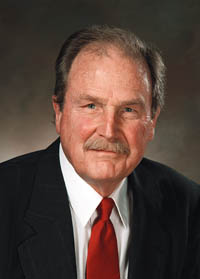
\includegraphics[height = 0.7in, width = 0.65in]{images/huffman.jpg} & 
		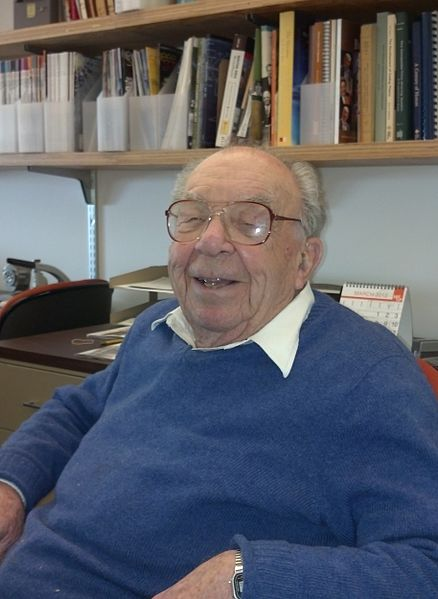
\includegraphics[height = 0.7in, width = 0.65in]{images/fano.jpg} & 
		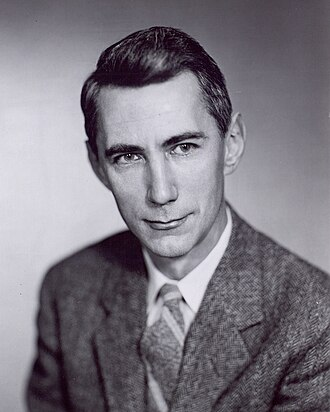
\includegraphics[height = 0.7in, width = 0.65in]{images/shannon.jpg} \\
		\scriptsize{David A. Huffman} & \scriptsize{Robert M. Fano} & \scriptsize{Claude Shannon} \\
	\end{tabular} 
	\caption{Pioneers in developing compression techniques}
	\end{figure}   
\end{center}

In doing so, Huffman outdid Fano, who alongside Claude Shannon developed
a similar method. Huffman’s bottom-up approach turned out to be more
optimal than the top-down approach of Shannon and Fano.

\newpage

\section{Applications}

Huffman coding is used in multifaceted applications where data compression is necessary. Some of those applications are: 

\begin{itemize}
	\item \textbf{File Compression:} Huffman coding is widely utilized in file compression algorithms like ZIP, gzip, and zlib. Inferring the approximate distribution of characters over a large file, Huffman's algorithm assigns variable-length codes to encode the file, thereby reducing the size to a significant extent. 
	
	\item \textbf{Text Compression:}  Huffman coding finds applications in compressing textual data such as ASCII text and HTML documents. By reducing the size of text files, it optimizes storage space and transmission bandwidth. 
	
	\item \textbf{Image Compression:} In image compression standards like JPEG and PNG, Huffman coding is employed as part of entropy encoding to reduce redundancy in image data. 
	JPEG uses Huffman coding with Discrete Cosine Transform to compress data efficiently while maintaining image quality.
	
	\item \textbf{Audio Compression:} In audio compression formats like MP3 and AAC, Huffman coding is used to encode frequency deviations. Psychoacoustic modelling helps discard less significant portions of an audio, thereby reducing the size and preserving the perceived quality.
	
	
	\item \textbf{Network Communication:} Reducing the size of data packets transmitted over networks is crucial for optimzed data transfer and bandwidth utilization in network communication. Huffman coding reduces the size of data packets, leading to faster transmission times and reduced network congestion.
	
	
\end{itemize}

\newpage

\section{The Problem Definition}

Efficient digital communication requires converting any type of
information into binary strings. Since resource is limited, we must find
out a way of conversion such that the message requires least possible
bandwidth to transmit.

A computaionally specific definition of the problem is as follows.

\textbf{Find an encoding scheme that requires
minimum bits on average to encode a message.}

However, merely encoding a message is of no use unless it is computationally feasible to decode it in a reasonable amount of time and space. Therefore, the scheme must also have unique decodability. To ensure unique decodability, the encoding must be prefix-free. In other words, if $b_1$ and $b_2$ are the binary codes for the characters $c_1$ and $c_2$ respectively, it is required that, $b_1$ is not a prefix of $b_2$ and $b_2$ is not a prefix of $b_1$.



\section{A Naive Solution}

Say, for instance, we forget the requirement of optimality and design the simplest possible encoding scheme. We assign random binary strings of a fixed length to each of the characters. Note that, assigning distinct codes of the same length automatically ensures unique decodability.

Let's assume, the alphabet consists of the letters A, B, C, D, and E. Since there are 5 characters, we need at least 3 bits to uniquely encode each of them. So, we may randomly assign 3-bit binary strings from \textbf{000} to \textbf{100}

Doing so, we obtain the following table.

\begin{table}[h]
	\centering
	\begin{tabular}{|c|c|}
		\hline
		\textbf{Letter} & \textbf{Binary Code} \\
		\hline
		A & 000  \\
		%				\hline
		B & 001  \\
		%				\hline
		C & 010 \\
		%				\hline
		D & 011 \\
		%				\hline
		E & 100 \\
						\hline
	\end{tabular}
	\caption{Binary codes for naive encoding scheme}
\end{table}

Now, we may encode any string into a binary message with the help of the table.

While encoding, each of the letters in the string needs 3 bits to encode. Therefore, if the length of a message = $n$, the expected length of the binary code = $3n$

Average number of bits required per character = $\frac{3n}{n} = 3$

\newpage

\section{Huffman's Algorithm}

\subsection{The Idea}

David A. Huffman, in 1952, came up with a different idea for tackling the problem and it was proven by means of information theory that the output of his algorithm is guaranteed to be optimal. 

As we have already seen, the naive algorithm randomly assigns binary codes of same length for each character of the alphabet. Therefore, if there are $c$ characters in the alphabet, the minimum length of each of the codes is $log_{2}{c}$. Huffman, however, looked into the fact that assigning shorter codes for characters that occur more frequently in the language helps decrease the
average length of the encoded message, thereby reducing the cost of the transfer.

Based on the observation, Huffman proposed a greedy algorithm which builds a tree in bottom-up order by maintaining a priority queue of characters based on their relative frequencies. This tree, once built, can be used to encode or decode any string of the language.

\subsection{Steps}

\begin{enumerate}
	\item Maintain a min-heap of nodes for characters with their relative frequencies as weights. 
	
	\item Pop two nodes with minimum weights 
	
	\item Merge them into a single node whose weight will be the summation of the previous nodes
	
	\item Push the newly created node back into the min-heap
	
	\item Repeat until the min-heap contains only the root of the tree
	
	\item Use the Huffman tree to encode any message
	
\end{enumerate}

\subsection{Pseudocode}

\begin{algorithm}[H]
	\SetAlgoLined
	\DontPrintSemicolon
	\SetKwFunction{Huffman}{Huffman}
	\SetKwProg{Fn}{Function}{}{end}
	\Fn{\Huffman{$f[1..n]$}}{
		$Q \leftarrow$ priority queue containing all characters with their frequencies from $f$\;
		\For{$i \leftarrow 1$ \KwTo $n-1$}{
			allocate a new node $z$\;
			$z.left \leftarrow x \leftarrow$ Extract-Min($Q$)\;
			$z.right \leftarrow y \leftarrow$ Extract-Min($Q$)\;
			$z.freq \leftarrow x.freq + y.freq$\;
			Insert($Q, z$)\;
		}
		\Return{the root of the tree}\;
	}
	\caption{Huffman's Algorithm}
\end{algorithm}

\subsection{Properties}

\begin{itemize}
	
	\item \textbf{Greedy Choice Property:} At each step, we choose the two \textbf{least probable} symbols and merge them into a single node with a combined probability.
	
	\item \textbf{Optimal Substructure:} The optimal solution to the entire problem can be constructed from optimal solutions to its subproblems. When we merge two nodes and treat it just like leaf nodes subsequently, we essentially rely on this property.
	
\end{itemize}

\subsection{The Intuition}

The reason why the greedy approach gurantees optimality in the problem lies in the fact that the algorithm always places more-frequent characters closer
to the root of the tree reducing the distance of these nodes from root and thereby decreasing the length of the binary encoding for them.

Since we always pop two nodes with minimum frequencies from the priority queue and merge them to form a new node, it is ensured that, less-frequent characters are placed farther from the root and vice versa. Furthermore, as we will explore later, the binary encoding of a character is derived bit by bit while traversing the tree from root to the desired character in a top-down manner. Therefore, the distance of a character from the root in the tree directly correlates with the length of the binary encoding.

The tree structure is necessary for ensuring a prefix-free encoding. It is evident that, the path from the root to a certain leaf can never be the prefix of the path to a different leaf of a binary tree must not have any common prefix with each other because at some internal node of the tree, a branching must have separated them and therefore there must be at least one additional character in both of the paths after the common prefix.


\section{The Huffman Tree}

In Huffman encoding, symbols are represented by nodes in a binary
tree structure which is named the Huffman Tree. It is built using a bottom-up greedy approach.

Nodes of a Huffman Tree are associated with frequency values that represent the sum of the the frequencies of the characters in the corresponding subtree. Edges are used to decide which bit to append to the binary encoding of a character at the corresponding step.

\subsection{Properties}

\begin{itemize}
	\item Symbols are represented by \textbf{leaves} in a binary tree structure.
	\item Each symbol in the tree has a \textbf{unique path} from the root to its corresponding leaf node.
	\item The path consists of left (0) and right (1) branches, \textbf{uniquely} identifying each symbol.
	\item Ensures \textbf{prefix-free} encoding.
\end{itemize}

\subsection{Construction of Huffman Tree}

Given the characters of a language with their relative frequencies, we can construct a Huffman Tree following the steps mentioned in the algorithm. Let us go through a simulation demonstrating the process.

Assume, a certain language consists of 5 characters A, B, C, D, and E. Let us define the relative frequency of a certain character as the number of times it appears in a sample text divided by the total number of characters in the same. Say, for instance, we observe that, in a large text of 1 million characters, $A$ appears 170 thousand times. Therefore, relative frequency of $A$ $ = \frac{170000}{1000000} = 0.17$


In a similar manner, we tabulate the relative frequencies of each of the characters.


\begin{table}[h]
	\centering
	\begin{tabular}{|c|c|}
		\hline
		\textbf{Letter} & \textbf{Relative Frequency} \\
		\hline
		A & 0.17  \\
						\hline
		B & 0.35  \\
						\hline
		C & 0.17 \\
						\hline
		D & 0.15 \\
						\hline
		E & 0.16 \\
						\hline
			
	\end{tabular}
	\caption{Relative frequencies of characters}
\end{table}
	

\textbf{Step 1:} First we push all the characters to the min-heap with their relative frequencies as weights.

\begin{figure}[h]

\centering
\leafnode{leafcolorone}{leafcolortwo}{black}{0.15}{D}{010}
\leafnode{leafcolorone}{leafcolortwo}{black}{0.16}{E}{011}
\leafnode{leafcolorone}{leafcolortwo}{black}{0.17}{A}{000}
\leafnode{leafcolorone}{leafcolortwo}{black}{0.17}{C}{001}
\leafnode{leafcolorone}{leafcolortwo}{black}{0.35}{B}{1}

\end{figure}

Here, the minimum weighted two nodes are $D(0.15)$ and $E(0.16)$. 

\textbf{Step 2:} Upon merging $D(0.15)$ and $E(0.16)$, we obtain an internal node with weight $0.31$.


\begin{figure}[h]
	\centering
	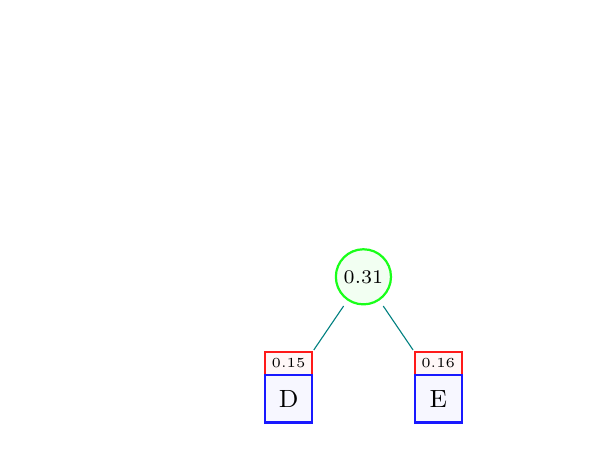
\begin{tikzpicture}[
		level distance=\leveldistance
		]
		
		\node {\internalnode{white}{white}{1.00}}
		child[noedge]{
			node {\internalnode{white}{white}{0.65}}
			child[noedge]{
				node {\internalnode{white}{white}{0.34}}
				child[noedge]{
					node {\leafnode{white}{white}{white}{0.17}{A}{000}}
				}
				child[noedge]{
					node {\leafnode{white}{white}{white}{0.17}{C}{001}}
				}
			}
			child[noedge]{
				node {\internalnode{internalnodecolor}{black}{0.31}}
				child[norm]{
					node {\leafnode{leafcolorone}{leafcolortwo}{black}{0.15}{D}{010}}
				}
				child[norm]{
					node {\leafnode{leafcolorone}{leafcolortwo}{black}{0.16}{E}{011}}
				}
			}
		}
		child[noedge]{
			node {\leafnode{white}{white}{white}{0.35}{B}{1}}
		};
		
	\end{tikzpicture}
	\caption{State of the tree after first merge}
\end{figure}

\newpage

We push the newly created node back into the min-heap. 

\begin{figure}[h]

\centering
\leafnode{leafcolorone}{leafcolortwo}{black}{0.17}{A}{000}
\leafnode{leafcolorone}{leafcolortwo}{black}{0.17}{C}{001}
\internalnode{internalnodecolor}{black}{0.31}
\leafnode{leafcolorone}{leafcolortwo}{black}{0.35}{B}{1}

\end{figure}

Now the minimum weighted two nodes turn out to be $A(0.17)$ and $C(0.17)$.

\textbf{Step 3:} After merging $A(0.17)$ and $C(0.17)$, we obtain a new internal node with weight $0.34$.

\begin{figure}[h]
	\centering
	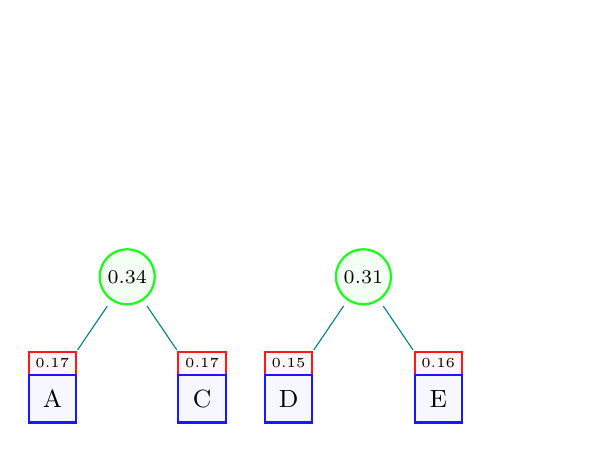
\begin{tikzpicture}[
		level distance=\leveldistance
		]
		
		\node {\internalnode{white}{white}{1.00}}
		child[noedge]{
			node {\internalnode{white}{white}{0.65}}
			child[noedge]{
				node {\internalnode{internalnodecolor}{black}{0.34}}
				child[norm]{
					node {\leafnode{leafcolorone}{leafcolortwo}{black}{0.17}{A}{000}}
				}
				child[norm]{
					node {\leafnode{leafcolorone}{leafcolortwo}{black}{0.17}{C}{001}}
				}
			}
			child[noedge]{
				node {\internalnode{internalnodecolor}{black}{0.31}}
				child[norm]{
					node {\leafnode{leafcolorone}{leafcolortwo}{black}{0.15}{D}{010}}
				}
				child[norm]{
					node {\leafnode{leafcolorone}{leafcolortwo}{black}{0.16}{E}{011}}
				}
			}
		}
		child[noedge]{
			node {\leafnode{white}{white}{white}{0.35}{B}{1}}
		};
		
	\end{tikzpicture}
	\caption{State of the tree after second merge}
\end{figure}


We again push the newly created internal node back into the min-heap.

\begin{figure}[h]

\centering
\internalnode{internalnodecolor}{black}{0.31}
\internalnode{internalnodecolor}{black}{0.34}
\leafnode{leafcolorone}{leafcolortwo}{black}{0.35}{B}{1}

\end{figure}

After this step, the nodes to be popped from the min-heap are the two internal nodes with weights $0.34$ and $0.31$. These nodes will now be merged.

\newpage

\textbf{Step 4:} Merging the internal nodes with weights $0.34$ and $0.31$, a new internal node with weight $0.65$ is created.


\begin{figure}[h]
	\centering
	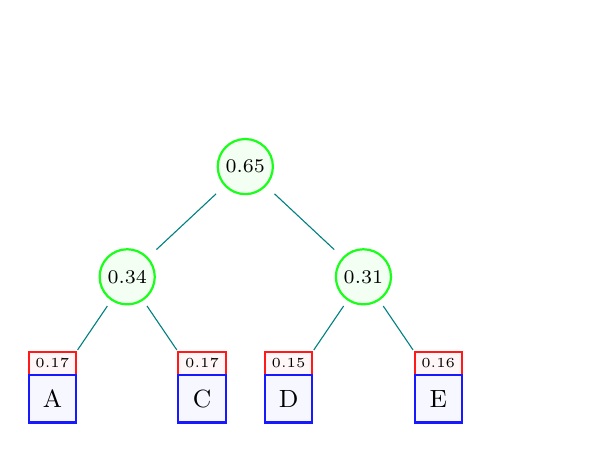
\begin{tikzpicture}[
		level distance=\leveldistance
		]
		
		\node {\internalnode{white}{white}{1.00}}
		child[noedge]{
			node {\internalnode{internalnodecolor}{black}{0.65}}
			child[norm]{
				node {\internalnode{internalnodecolor}{black}{0.34}}
				child[norm]{
					node {\leafnode{leafcolorone}{leafcolortwo}{black}{0.17}{A}{000}}
				}
				child[norm]{
					node {\leafnode{leafcolorone}{leafcolortwo}{black}{0.17}{C}{001}}
				}
			}
			child[norm]{
				node {\internalnode{internalnodecolor}{black}{0.31}}
				child[norm]{
					node {\leafnode{leafcolorone}{leafcolortwo}{black}{0.15}{D}{010}}
				}
				child[norm]{
					node {\leafnode{leafcolorone}{leafcolortwo}{black}{0.16}{E}{011}}
				}
			}
		}
		child[noedge]{
			node {\leafnode{white}{white}{white}{0.35}{B}{1}}
		};
		
	\end{tikzpicture}
	\caption{State of the tree after third merge}
\end{figure}


After we push this node back, the min-heap reaches the following state.

\begin{figure}[h]

\centering
\leafnode{leafcolorone}{leafcolortwo}{black}{0.35}{B}{1}
\internalnode{internalnodecolor}{black}{0.65}

\end{figure}

The only two remaining nodes will be merged.


\textbf{Step 5:} After performing the final merge, we obtain the complete huffman tree. Note that, the weight associated with the root of the tree turns out to be $1.00$, just as expected.



\begin{figure}[h]
	\centering
	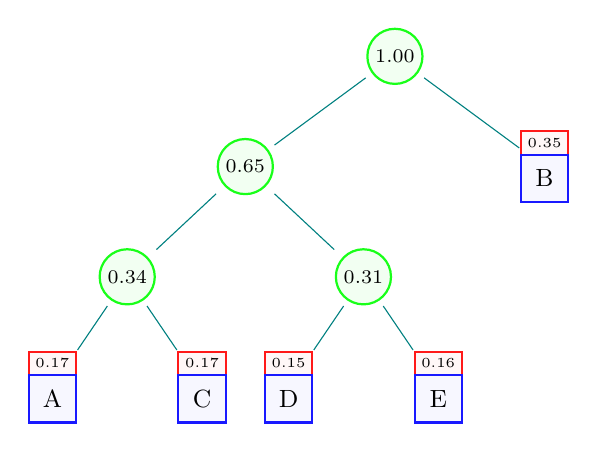
\begin{tikzpicture}[
		level distance=\leveldistance
		]
		
		\node {\internalnode{internalnodecolor}{black}{1.00}}
		child[norm]{
			node {\internalnode{internalnodecolor}{black}{0.65}}
			child[norm]{
				node {\internalnode{internalnodecolor}{black}{0.34}}
				child[norm]{
					node {\leafnode{leafcolorone}{leafcolortwo}{black}{0.17}{A}{000}}
				}
				child[norm]{
					node {\leafnode{leafcolorone}{leafcolortwo}{black}{0.17}{C}{001}}
				}
			}
			child[norm]{
				node {\internalnode{internalnodecolor}{black}{0.31}}
				child[norm]{
					node {\leafnode{leafcolorone}{leafcolortwo}{black}{0.15}{D}{010}}
				}
				child[norm]{
					node {\leafnode{leafcolorone}{leafcolortwo}{black}{0.16}{E}{011}}
				}
			}
		}
		child[norm]{
			node {\leafnode{leafcolorone}{leafcolortwo}{black}{0.35}{B}{1}}
		};
		
	\end{tikzpicture}
	\caption{Obtained Huffman Tree}
\end{figure}

\newpage

\subsection{Interpretation of Huffman Tree}

Now let us understand how to interpret binary encodings from the Huffman Tree.

Let’s say we want to find the binary encoding of the letter $D$.

First we need to find a path from the root to the leaf containing $D$. For every left
branch, we append a $0$ and for every right branch, we append a $1$ to
the binary encoding.

The traversal is depicted in the following figure.


\begin{figure}[h]
	\centering
	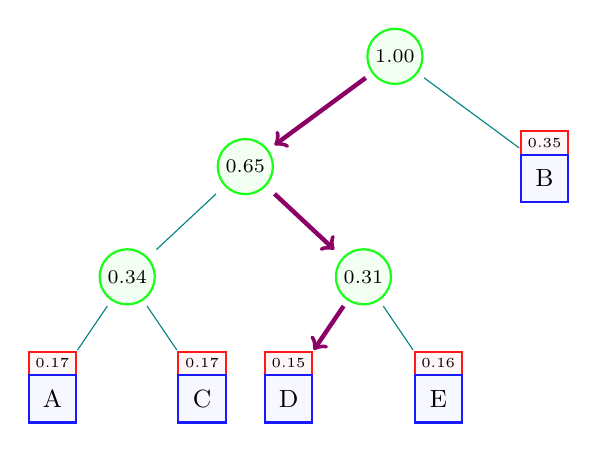
\begin{tikzpicture}[
		level distance=\leveldistance
		]
		
		\node {\internalnode{internalnodecolor}{black}{1.00}}
		child[emph]{
			node {\internalnode{internalnodecolor}{black}{0.65}}
			child[norm]{
				node {\internalnode{internalnodecolor}{black}{0.34}}
				child[norm]{
					node {\leafnode{leafcolorone}{leafcolortwo}{black}{0.17}{A}{000}}
				}
				child[norm]{
					node {\leafnode{leafcolorone}{leafcolortwo}{black}{0.17}{C}{001}}
				}
			}
			child[emph]{
				node {\internalnode{internalnodecolor}{black}{0.31}}
				child[emph]{
					node {\leafnode{leafcolorone}{leafcolortwo}{black}{0.15}{D}{010}}
				}
				child[norm]{
					node {\leafnode{leafcolorone}{leafcolortwo}{black}{0.16}{E}{011}}
				}
			}
		}
		child[norm]{
			node {\leafnode{leafcolorone}{leafcolortwo}{black}{0.35}{B}{1}}
		};
		
	\end{tikzpicture}
	\caption{Interpretation of Huffman Tree for the character $D$}
\end{figure}

Since, we followed left($0$), right($1$) and left($0$) branch respectively,  the binary encoding of $D$ = \textbf{$010$}

In a similar manner, we tabulate the binary codes for all the characters.

\begin{table}[h]
	\centering
	\begin{tabular}{|c|c|}
		\hline
		\textbf{Letter} & \textbf{Binary Code} \\
		\hline
		A & 000  \\
		%				\hline
		B & 1  \\
		%				\hline
		C & 001 \\
		%				\hline
		D & 010 \\
		%				\hline
		E & 011 \\
						\hline
	\end{tabular}
	\caption{Binary codes interpreted from the Huffman Tree}
\end{table}


\subsection{Comparison}

In our naive encoding scheme described earlier, the average length of the binary encoding of a character $3$. Now let’s calculate the same for the above table obtained from the Huffman Tree.

Since expected value is additive, we obtain,

Average Length = $0.17 \times 3 + 0.35 \times 1 + 0.17 \times 3 + 0.15 \times 3 + 0.16 \times 3$ = $2.3$

Now we calculate the compression ratio,

Compression ratio = $\frac{3-2.3}{3} \times 100 \% = \textbf{23.33 \%} $

\newpage

\section{Encoding}

Encoding refers to the process of converting a string into a binary message under a certain scheme or strategy. As we have seen earlier, the Huffman Tree helps us determine the binary codes for each of the characters of a language. Encoding a string is fairly straightforward. We just need to scan the input string from left to right and upon encountering a character, wee need to look up its code and append it to the binary message.

\subsection{An Example}

For convenience, the previously obtained table is again presented here.

\begin{table}[h]
	\centering
	\begin{tabular}{|c|c|}
		\hline
		\textbf{Letter} & \textbf{Binary Code} \\
		\hline
		A & 000  \\
		%				\hline
		B & 1  \\
		%				\hline
		C & 001 \\
		%				\hline
		D & 010 \\
		%				\hline
		E & 011 \\
		\hline
	\end{tabular}
\end{table}

Let us assume we want to encode the string $DECADE$ with Huffman Encoding following the above mentioned table. The following figure demonstrates how we obtain the encoded message.

\begin{center}
	\Large
	\textcolor{codecolorone}{\textbf{D}}
	\textcolor{codecolortwo}{\textbf{E}}
	\textcolor{codecolorone}{\textbf{C}}
	\textcolor{codecolortwo}{\textbf{A}}
	\textcolor{codecolorone}{\textbf{D}}
	\textcolor{codecolortwo}{\textbf{E}}
\end{center}

\begin{center}
	\huge
	\textcolor{codecolorone}{\textbf{010}}
	\textcolor{codecolortwo}{\textbf{011}}
	\textcolor{codecolorone}{\textbf{001}}
	\textcolor{codecolortwo}{\textbf{000}}
	\textcolor{codecolorone}{\textbf{010}}
	\textcolor{codecolortwo}{\textbf{011}}
\end{center}

Thus we obtain the binary encoding of the string $DECADE$ = $\textbf{010011001000010011}$

\subsection{Efficiency of Encoding}

According to Information Theory,

\[
\text{Entropy}, H = - \sum_{i=1}^{n} p_i \cdot \log_2(p_i)
\]

Here $p_i$ denotes the probability of the occurrence of the $i$th symbol. For our word $DECADE$, we calculate entropy as follows-

\begin{align*}
	H = & - (0.17 \cdot \log_2(0.17) \\
	& + 0.35 \cdot \log_2(0.35) \\
	& + 0.17 \cdot \log_2(0.17) \\
	& + 0.15 \cdot \log_2(0.15) \\
	& + 0.16 \cdot \log_2(0.16)) = 2.23 \\
\end{align*}

We know, 

\[
\text{Efficiency} = \frac{\text{Entropy}}{\text{Number of bits per symbol}} \times 100 \%
\]
$$$$
Encoding of our word "DECADE" is - 010 011 001 000 010 011
\\\\
Number of bits per symbol = $\frac{18}{6} = 3$
$$$$
\[
\text{Efficiency} = \frac{2.23}{3}\times 100\% = \textbf{74.33\%}
\]


\newpage

\section{Decoding}

Since we have the binary codes for all the characters, one simple strategy for decoding would be to perform a reverse-lookup for prefixes of the binary message until we find a matching character, and thereby decoding the string letter by letter. This approach, however is neither computationally efficient not conceptually interesting.

Instead, we may just resort to the Huffman Tree. The traversal starts from the root and proceeds in a top-down manner. Just as we interpreted edges of the tree previously, upon having a \textbf{0}, we turn \textbf{left} and upon having a \textbf{1}, we turn \textbf{right} until we reach a leaf. When we reach a leaf, the corresponding character is appended to the decoded message and thus the string is decoded character by character.


\subsection{An Example}

Assume we need to decode the binary message \textbf{1011011}. The steps proceed as follows.

\textbf{Step 1:} First we encounter a \textbf{1} and upon turning right, we reach a leaf containing \textbf{B}. Thus we add \textbf{B} to the decoded string.

\begin{center}
	\begin{table}[h]
		\centering
		\begin{tabular}{cc}
			\huge{\textcolor{codecolorone}{\textbf{1}}} \huge{\textcolor{dimcolor}{\textbf{011011}}} & \huge{\textbf{B}} \\
		\end{tabular}
		\label{tab:my_label}
	\end{table}
\end{center}

\begin{figure}[h]
	\centering
	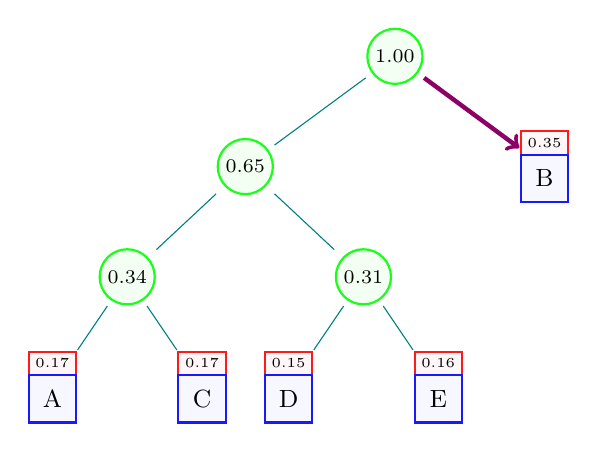
\begin{tikzpicture}[
		level distance=\leveldistance
		]
		
		\node {\internalnode{internalnodecolor}{black}{1.00}}
		child[norm]{
			node {\internalnode{internalnodecolor}{black}{0.65}}
			child[norm]{
				node {\internalnode{internalnodecolor}{black}{0.34}}
				child[norm]{
					node {\leafnode{leafcolorone}{leafcolortwo}{black}{0.17}{A}{000}}
				}
				child[norm]{
					node {\leafnode{leafcolorone}{leafcolortwo}{black}{0.17}{C}{001}}
				}
			}
			child[norm]{
				node {\internalnode{internalnodecolor}{black}{0.31}}
				child[norm]{
					node {\leafnode{leafcolorone}{leafcolortwo}{black}{0.15}{D}{010}}
				}
				child[norm]{
					node {\leafnode{leafcolorone}{leafcolortwo}{black}{0.16}{E}{011}}
				}
			}
		}
		child[emph]{
			node {\leafnode{leafcolorone}{leafcolortwo}{black}{0.35}{B}{1}}
		};
		
	\end{tikzpicture}
	\caption{Traversal while decoding the first character}
\end{figure}

\newpage

\textbf{Step 2:} Then we keep moving down the tree for three additional bits and reach a reach containing \textbf{E}. Thus, our decoded string becomes \textbf{BE} so far.

\begin{center}
	\begin{table}[h]
		\centering
		\begin{tabular}{lr}
			\huge{\textcolor{codecolortwo}{\textbf{1}}}
			\huge{\textcolor{codecolorone}{\textbf{011}}} \huge{\textcolor{dimcolor}{\textbf{011}}} 
			\hspace{2mm}
			& 
			\hspace{2mm}
			\huge{\textcolor{codecolortwo}{\textbf{B}}}
			\huge{\textcolor{codecolorone}{\textbf{E}}}
			\\
		\end{tabular}
		\label{tab:my_label}
	\end{table}
\end{center}

\begin{figure}[h]
	\centering
	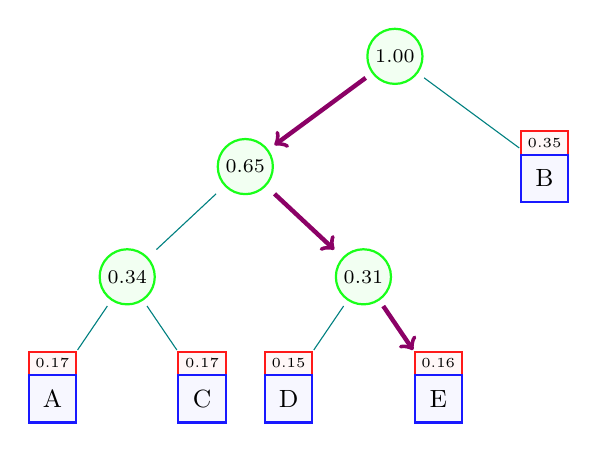
\begin{tikzpicture}[
		level distance=\leveldistance
		]
		
		\node {\internalnode{internalnodecolor}{black}{1.00}}
		child[emph]{
			node {\internalnode{internalnodecolor}{black}{0.65}}
			child[norm]{
				node {\internalnode{internalnodecolor}{black}{0.34}}
				child[norm]{
					node {\leafnode{leafcolorone}{leafcolortwo}{black}{0.17}{A}{000}}
				}
				child[norm]{
					node {\leafnode{leafcolorone}{leafcolortwo}{black}{0.17}{C}{001}}
				}
			}
			child[emph]{
				node {\internalnode{internalnodecolor}{black}{0.31}}
				child[norm]{
					node {\leafnode{leafcolorone}{leafcolortwo}{black}{0.15}{D}{010}}
				}
				child[emph]{
					node {\leafnode{leafcolorone}{leafcolortwo}{black}{0.16}{E}{011}}
				}
			}
		}
		child[norm]{
			node {\leafnode{leafcolorone}{leafcolortwo}{black}{0.35}{B}{1}}
		};
		
	\end{tikzpicture}
	\caption{Traversal while decoding the second character}
\end{figure}



\textbf{Step 3:} The rest of the string is again \textbf{011}. So it will also be decoded as \textbf{E}.


\begin{center}
	\begin{table}[h]
		\centering
		\begin{tabular}{lr}
			\huge{\textcolor{codecolortwo}{\textbf{1011}}}
			\huge{\textcolor{codecolorone}{\textbf{011}}} \huge{\textcolor{dimcolor}{\textbf{}}} 
			\hspace{2mm}
			& 
			\hspace{2mm}
			\huge{\textcolor{codecolortwo}{\textbf{BE}}}
			\huge{\textcolor{codecolorone}{\textbf{E}}}
			\\
		\end{tabular}
		\label{tab:my_label}
	\end{table}
\end{center}

Thus, out decoded string turns out to be \textbf{BEE}.

\newpage

\section{Time Complexity Analysis}

\subsection{Building Frequency Table}

To construct the Huffman Tree, we first need the relative frequency values of each of the characters. To do this, we may simply maintain a count-array while scanning a large input text from first to last.

Thus, if the number of symbols in the input = $n$, Time Complexity = $\textbf{O(n)}$

\subsection{Building The Huffman Tree}

Assume there are $n$ distinct symbols in the language. Then the running time complexity of the construction of Huffman Tree is determined as follows.

\begin{description}
	
	\item[1. Constructing Initial Heap] 
	Although a single insertion to a heap takes $O(logn)$ time, a heap can be constructed bottom-up in $O(n)$ time from the frequency table obtained earlier. Therefore,
	
	Time Complexity = $\textbf{O(n)}$
	
	\item[2. Merging Nodes in the Heap] 
	Every merge requires two extract-min operations on the min-heap. If there are $n$ distinct symbols in the language, $O(n)$ merges are needed in total. Since an extract-min operation takes $O(logn)$ time, 
	
	Time Complexity = $\textbf{O(nlogn)}$
	
\end{description}

\subsection{Generating Huffman Codes}
Once we have obtained the Huffman Tree, determining the huffman encodings of the characters needs traversing the tree in a top-down manner. This can be done with any tree-traversal algorithm like BFS or DFS.

Time Complexity = $\textbf{O(n)}$

\subsection{Encoding a Message}

While scanning the input message from left to right, for each character, we need to append the corresponding binary code to the encoded binary message. Therefore, if the length of the input text is $n$ and the average length of the encoding of a character is $k$, 

Time Complexity = $\textbf{O(nk)}$

\subsection{Decoding a Message}

Once the Huffman Tree has been built, decoding only requires traversing the tree one edge per input bit. Thus if the encoded binary string has $n$ bits,

Time Complexity = $\textbf{O(n)}$


\newpage


\section{Conclusion}

In conclusion, Huffman coding has been a fundamental stepping
stone in the journey of data compression. It revolutionized the field by providing efficient and effective
compression techniques based on symbol frequencies. Despite the emergence of more sophisticated compression
algorithms, Huffman coding remains widely used in various
applications.


\end{document}